\documentclass[a4paper,12pt]{article}
\usepackage{graphicx}
\usepackage{enumerate}
\usepackage{geometry}
\usepackage{times}
\geometry{legalpaper, portrait, margin=.75in}

\begin{document}

\begin{flushright}

\vspace{1.1cm}

{\bf\Huge Lab 4}

\rule{0.25\linewidth}{0.5pt}

\vspace{0.5cm}
%Put Authors
Justin Ely
\linebreak
\newline
%Put Author's affiliations
\footnotesize{615.202.81.FA15 Data Structures \\}
\vspace{0.5cm}
% Date here below
06 December, 2015
\end{flushright}

\noindent\rule{\linewidth}{1.0pt}

%%%%%%%%%%%%%%%%%%%%%%%%%%%%%%%%%%%%%%%%%%%%%%%%%%%%%%%%%%

\section{Comments}
Sorting algorithms are a key component to computer science, not simply because sorting is a commonly-performed task, but because there is a wealth of knowledge to be gained through examining the various algorithms.  The development and usage of the different methods clearly demonstrates how limiting any particular implementation can be, and the lengths that need to be employed to be truly useful in all scenarios.

In this lab we mainly explored two sorting algorithms, quick sort and heap sort, with additional analysis on insertion sort and various sub-implementations of quick sort.  From this exploration, we can see that the main factor in choosing a sorting algorithm is the number of elements to be sorted.  For small sorts any of the available methods will complete in fractions of a second, and would be a fine choice in anything but very optimized computations and repeated operations.  For larger file sizes however, the choice of algorithm can quickly change a solvable program into an insolvable one as the difference in execution times can vary by several orders of magnitude.  In addition, many sorting methods do show significant variations in their time-complexity growth-rate as a function of the initial ordering of the input data.  This effect can be eliminated with minor modifications to the internal workings of the algorithms in some instances.


%%%%%%%%%%%%%%%%%%%%%%%%%%%%%%%%%%%%%%%%%%%%%%%%%%%%%%%%%%

\section{Design}
\subsection{Recursion vs Iteration}
I chose to do both the heap sort and quick sort as recursive algorithms.  A main driver for this was that a recursive quick sort was a requirement for other parts of the lab.  By starting off with a recursive function, some extra work could be avoided.  Additionally, since quicksort and heapsort both can be easily understood in a recursive form, the development wasn't burdensome, and the extra time needed to come up with an iterative scheme could be dropped.


\subsection{Enhancements}
My first enhancement was driven by the recursive implementation of the quicksort.  The default stack size for the JVM was insufficient  to sort some of the larger input arrays, so an optional runtime flag was added to the Makefile to increase the size.  By running the Driver for quick sort with '-Xss200m', files of more than 10,000,000 items can be sorted.  

To get a better grasp of the time-complexity, and to see when these algorithms can truly become prohibitive, files with up to 1,000,000 items were included in the analysis.  Additionally, input files that contained large numbers of repeated values were analyzed, as this unique edge-case can cause significant problems to certain algorithms as well as show the robustness of the algorithm by not failing on duplicates in data. 

In addition to the recursive heap sort, a iterative version was completed as well.  This was done in an attempt to measure the amount of overhead introduced by a recursive function, but the differences proved too small to notice.  Though an insertion sort method was only required as part of the particular quick sort implementations, I separated out the implementation of insertion sort and included it's time-complexity in the analysis.  This provides a useful benchmark, as the algorithm is considerably simpler than any of the other methods employed.

Unittests were added and used throughout development.  This was crucial to ensuring that any modifications to the sorting algorithms didn't cause a disruption in their ability to correctly sort data.  Additionally, the javadoc tool was used to provide documentation to the project.  However, due to the use of non-standard libraries for these functions, the ability to disable them was added to the included makefile.


\subsection{Limitations}
The main limitation is the restriction to integer type.  Both the main driver and the individual sorting methods are all limited to work with integer values.  The main program will only read integers from the input files, and the sorting algorithms are hard-coded to build and work with integer arrays and comparisons.  

As discussed later in the Efficiency section, the current algorithms employed are a major limiting factor in the actual usefulness of the code.  Attempting to sort more than 1,000,000 items began to take multiple minutes to run, which limits the usefulness of the code.  Additionally, the space complexity of the standard quick sort algorithms limit the possible size of the input set to be sorted.  As discussed in Enhancements, many of the larger file sizes needed more space than the default stack allocation, and additional flags need to be set.  During testing, the maximum allowable heap size to the JVM was hit, which shows that there is even a limit to how much the memory can be expanded using the command-line flags.

%%%%%%%%%%%%%%%%%%%%%%%%%%%%%%%%%%%%%%%%%%%%%%%%%%%%%%%%%%

\section{Efficiency}

Tables, as well as a sequence of plots, of the various method's time efficiency can be found in the Timing Tables section.  From these timing measurements a few trends become clear, but what is most evident is how much variation in behavior is seen.

The one standout trend is that larger amounts of data take longer to sort.  Simple put, none of these algorithms have constant, $O(1)$, complexity, but rather they all grow with the input data size $(N)$.  However, the growth rate of each algorithm can be vastly different, with different dependencies on the initial ordering of the data.
 
Insertion sort is a very good sorting algorithm in only once case; when the data is already sorted.  In this instance, the growth rate is simply $O(N)$, and it is consistently the fastest sorting algorithm.  However, for any other sorting of the data (reverse, random, few unique) insertion sort was among the worst, with a growth rate of $O(n^2$).  At it's worst case it can be 4 orders of magnitude slower than the other available algorithms.

Quick sort displays an incredible range in performance across the various sortings.  The standard quick sort and quick sort with minimum partition sizes only perform well on random and few unique datasets.  For ordered and reversed, they actually perform on-par or worse than a simple insertion sort.  However, the quick sort variant that choses the pivot as the median-of-3 was the best performer across the various orderings and file sizes.  The median-of-3 version had a growth rate of $O(nlogn)$ accross all orderings.

The recursive quick sort employed also had a space efficiency problem.  The default stack size was not sufficient for the number of recursive calls employed, though this limitation was hit at lower file sizes with data that was initially ordered or reverse ordered.

Heap sort shows that it is a very good, all-purpose, sort.  For ordered, reverse, random, and few unique input datasets, there was no change in growth rate of $O(nlogn)$.  The time required often stayed factors of 1000 below the worst-performing algorithm. 

As discussed in the Enhancements section, both an iterative and recursive version of the heap sort was was implemented.  The analysis of the timing data for these two versions displays an interesting trend.  Though both versions show almost identical performance, for smaller datasets the iterative version is consistently faster than the recursive call.  This changes for larger datasets, where the recursive call becomes equal or faster than the iterative version.  This indicates that the recursive method may actually have slightly slower growth, but there is a small constant overhead that is only overcome with the larger file sizes.


%%%%%%%%%%%%%%%%%%%%%%%%%%%%%%%%%%%%%%%%%%%%%%%%%%%%%%%%%%

\section{What I learned}
The key take away from this lab is that sorting is not a "one size fits all" sort of problem.  From the timing alone, we can see that heap sort is a very good all-purpose sort.  Knowing nothing else, this would be a good sorting algorithm to employ.  However, if you know a little bit more about your input data, there are clear cases when a simpler method like insertion sort can actually be a much better solution.  Additionally, even an advanced sorting algorithm like like quick sort can have vastly improved performance with simple changes to some of the parameters.  Simply changing the pivot to median-of-3 vastly reduces the computation time required for already ordered datasets.

From experiencing the development of the algorithms first-hand, developer time and possibility of bugs is also a huge factor.  Though insertion sort is often much slower than the other sorting methods, the incredible simplicity of the coding makes it much easier and quicker to implement a robust version.

%%%%%%%%%%%%%%%%%%%%%%%%%%%%%%%%%%%%%%%%%%%%%%%%%%%%%%%%%%

\section{Next time}
The biggest change to make to the next iteration of the code would be to allow sorting of more than simply integers.  Through dynamic typing
and generic comparisons, floats and strings could also be sorted and compared.  Though the work done was sufficient for the requirements of the lab, expanding this functionality would allow the code to be of greater use in the future.  

For a more expansive understanding of the costs of various sort methods, I would also like to implement additional sorting methods.  In particular, shell sort and merge sort would be two algorithms that would be good to know and enlightening to benchmark.


%%%%%%%%%%%%%%%%%%%%%%%%%%%%%%%%%%%%%%%%%%%%%%%%%%%%%%%%%%


\section{Timing Tables}

Below are timing tables giving the running time for each algorithm on a given file size.  These tests were performed with a 4.0Ghz Intel Corei7 processor on a machine running Ubuntu 15.10.  All times are given in seconds.

\begin{figure}[h]
    \centering
    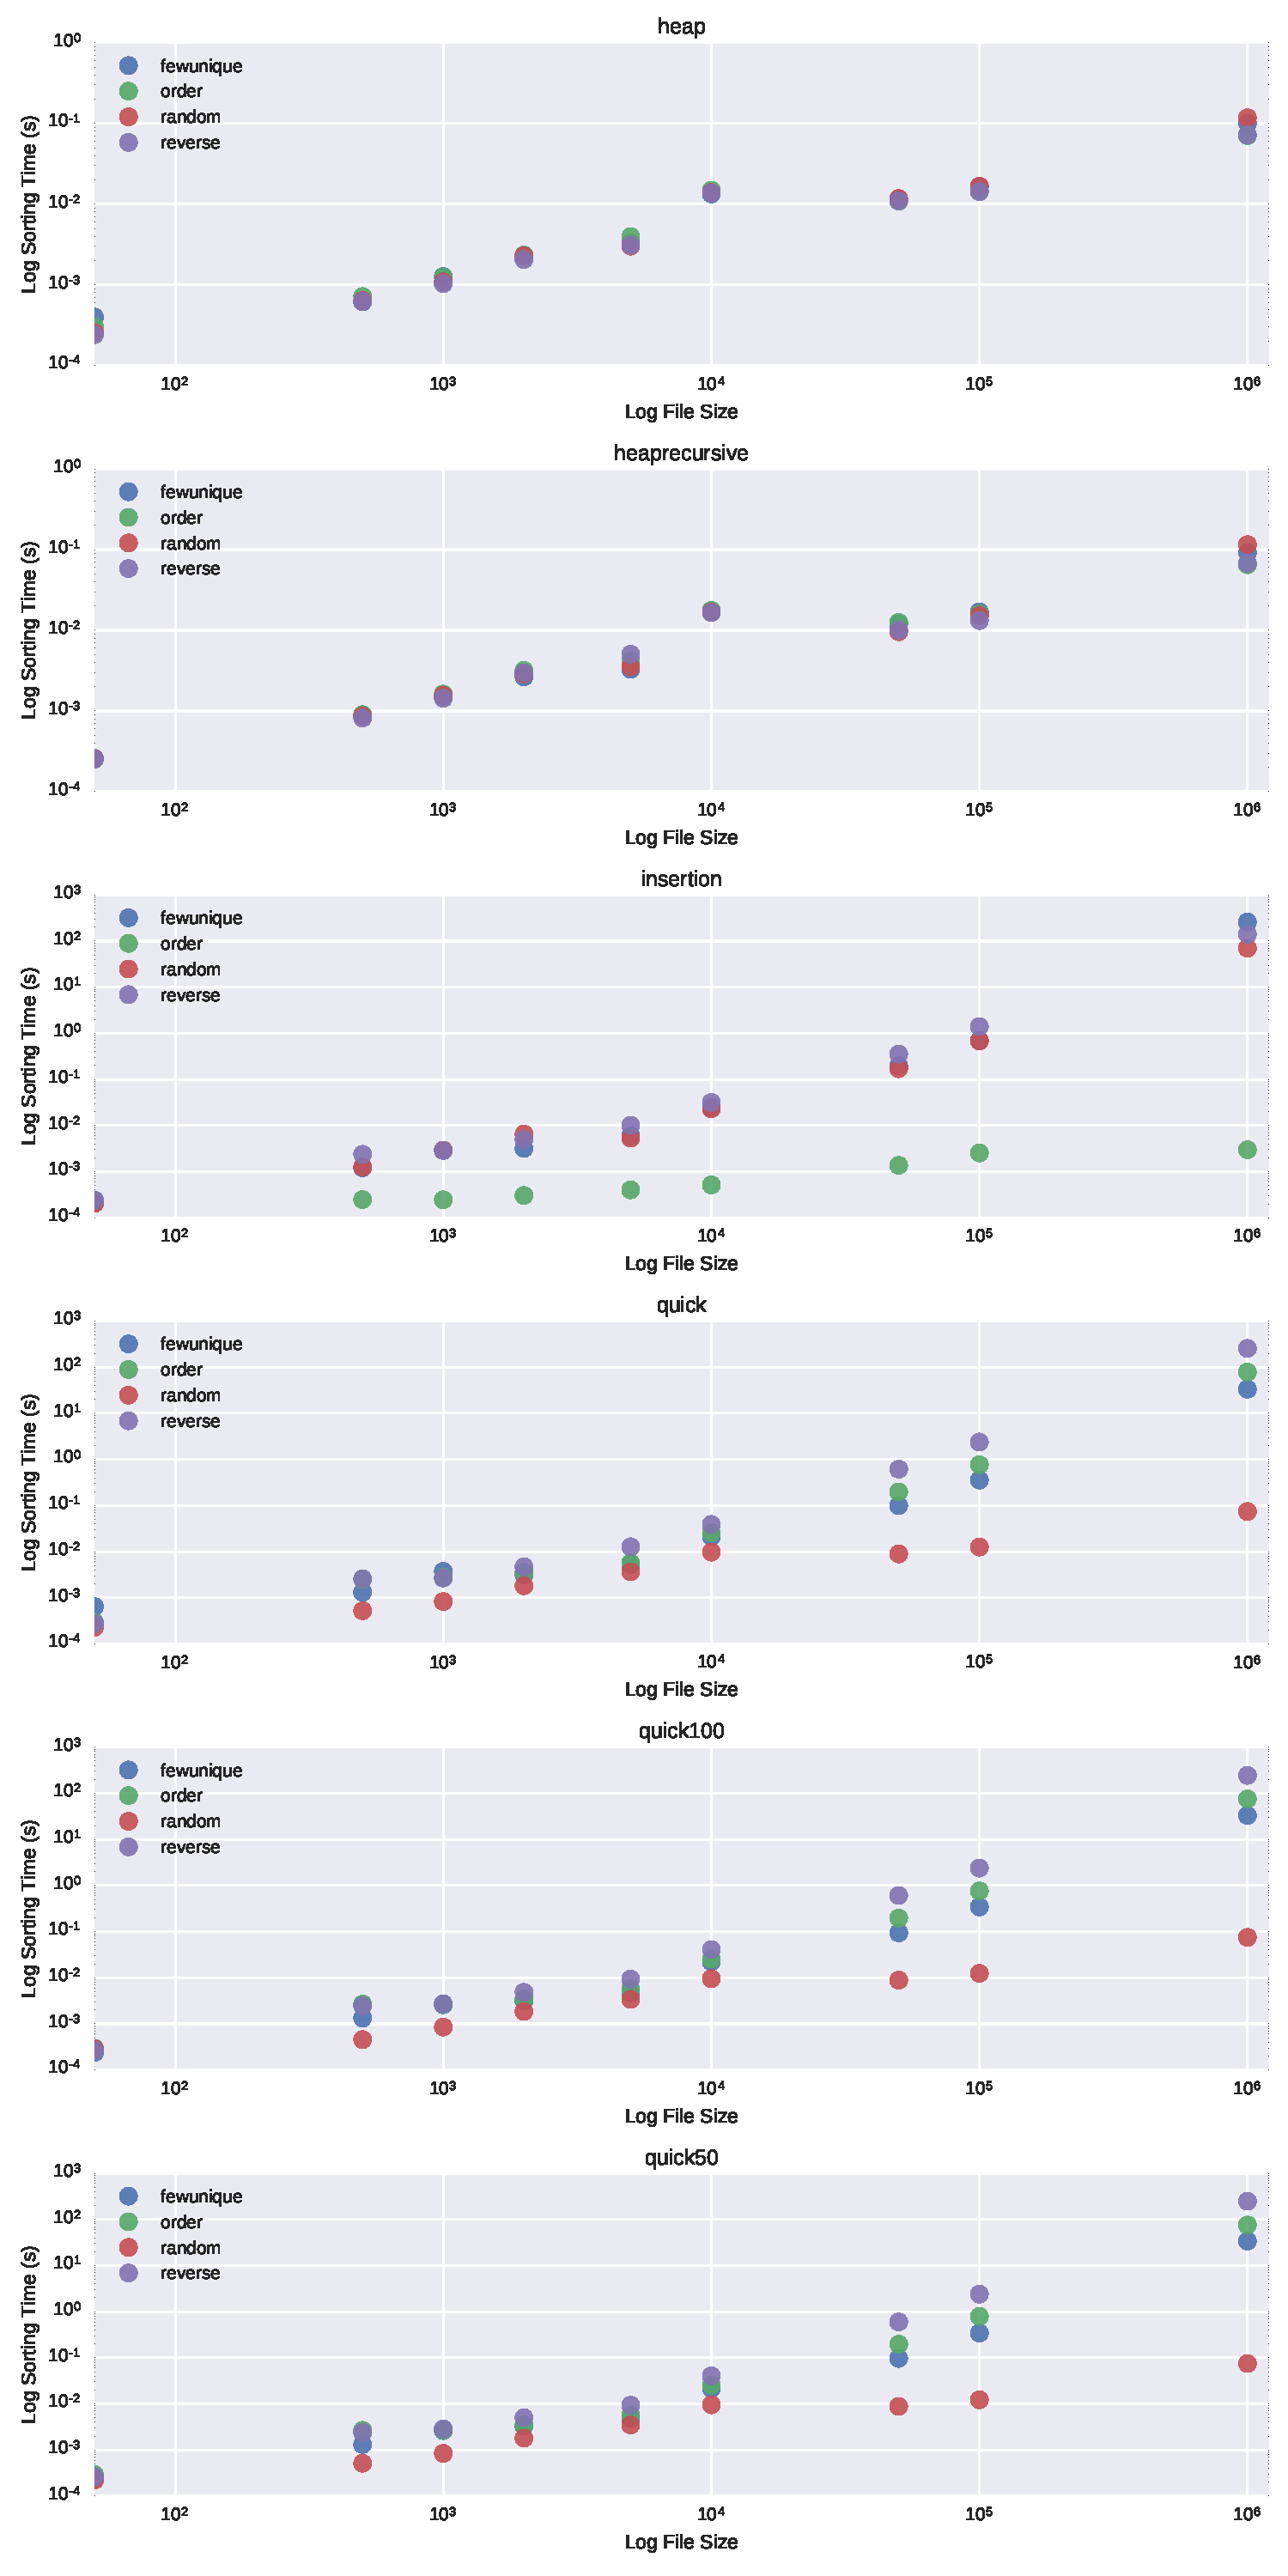
\includegraphics[width=.8\textwidth]{sorting_efficiency.pdf}
    \caption{Time complexity of the various sorting methods.  The order of the input dataset is marked as different colors, and is explained in the legend.  Note the variation in growth-rate at small sizes.  Heap is the iterative heap sort.  Heaprecursive is a recursive version of heap sort.  quick100 and quick50 are quick sorts where partitions below 100 and 50 elements, respectively, are sorted with an insertion sort.  Quickmed is a quick sort where the pivot is found as the median of 3.}
    \label{fig:mesh1}
\end{figure}


\begin{table}[h]
\caption {Ordered input data} 
\begin{tabular}{cccccccc}
size & heap & heaprecursive & insertion & quick & quick100 & quick50 & quickmed \\ \hline
50 & 0.000246 & 0.000256 & 0.000298 & 0.00022 & 0.000366 & 0.000372 & 0.000373 \\
500 & 0.000661 & 0.000905 & 0.000273 & 0.001541 & 0.001579 & 0.001622 & 0.00052 \\
1000 & 0.001061 & 0.001617 & 0.000305 & 0.002612 & 0.002859 & 0.002852 & 0.00071 \\
2000 & 0.002362 & 0.003185 & 0.000312 & 0.003778 & 0.003837 & 0.003775 & 0.00097 \\
5000 & 0.00465 & 0.004083 & 0.000405 & 0.009733 & 0.010107 & 0.010489 & 0.002566 \\
10000 & 0.013203 & 0.017161 & 0.001432 & 0.041087 & 0.039812 & 0.040178 & 0.005241 \\
50000 & 0.009149 & 0.012257 & 0.001532 & 0.690175 & 0.724731 & 0.741439 & 0.00828 \\
100000 & 0.013349 & 0.015266 & 0.001757 & 2.553904 & 2.775441 & 2.813958 & 0.012742 \\
1000000 & 0.065365 & 0.064342 & 0.004227 & 262.740136 & 267.217407 & 288.009517 & 0.029615 \\
\end{tabular}
\caption{Sorting time for the various methods on already sorted data.  All times are in seconds.}
\end{table}


\begin{table}[h]
\caption {Reversed input data} 
\begin{tabular}{cccccccc}
size & heap & heaprecursive & insertion & quick & quick100 & quick50 & quickmed \\ \hline
50 & 0.000263 & 0.00025 & 0.00022 & 0.000237 & 0.000374 & 0.000391 & 0.000374 \\
500 & 0.000615 & 0.000767 & 0.00247 & 0.001697 & 0.001838 & 0.001806 & 0.000587 \\
1000 & 0.000949 & 0.001374 & 0.002956 & 0.002694 & 0.00297 & 0.002993 & 0.000765 \\
2000 & 0.002002 & 0.00291 & 0.004888 & 0.00495 & 0.00506 & 0.004915 & 0.001029 \\
5000 & 0.002915 & 0.004976 & 0.007711 & 0.008681 & 0.008995 & 0.008888 & 0.002771 \\
10000 & 0.013201 & 0.016363 & 0.032004 & 0.032741 & 0.034495 & 0.033554 & 0.005503 \\
50000 & 0.010824 & 0.009857 & 0.380363 & 0.467297 & 0.453685 & 0.442681 & 0.006533 \\
100000 & 0.014268 & 0.013028 & 1.511343 & 1.808753 & 1.813493 & 1.809145 & 0.00865 \\
1000000 & 0.071608 & 0.06512 & 155.514205 & 181.413635 & 183.928399 & 194.786948 & 0.034295 \\
\end{tabular}
\caption{Sorting time for the various methods on reverse sorted data.  All times are in seconds.}
\end{table}

\begin{table}[h]
\caption {Random input data} 
\begin{tabular}{cccccccc}
size & heap & heaprecursive & insertion & quick & quick100 & quick50 & quickmed \\ \hline
50 & 0.000246 & 0.00026 & 0.000207 & 0.000226 & 0.00038 & 0.000374 & 0.000399 \\
500 & 0.000615 & 0.000824 & 0.00135 & 0.000437 & 0.000614 & 0.001069 & 0.000687 \\
1000 & 0.001036 & 0.001556 & 0.003327 & 0.000704 & 0.000892 & 0.000792 & 0.000895 \\
2000 & 0.002214 & 0.002829 & 0.003891 & 0.001242 & 0.001376 & 0.001139 & 0.001365 \\
5000 & 0.002997 & 0.003265 & 0.006122 & 0.003355 & 0.003185 & 0.002564 & 0.003556 \\
10000 & 0.012951 & 0.016346 & 0.025111 & 0.007254 & 0.005853 & 0.004879 & 0.007445 \\
50000 & 0.011191 & 0.009447 & 0.194281 & 0.010293 & 0.006654 & 0.007045 & 0.009257 \\
100000 & 0.015297 & 0.014491 & 0.812087 & 0.014799 & 0.01155 & 0.011501 & 0.014662 \\
1000000 & 0.108647 & 0.113197 & 81.490019 & 0.088074 & 0.078813 & 0.076101 & 0.091612 \\
\end{tabular}
\caption{Sorting time for the various methods on random sorted data.  All times are in seconds.}
\end{table}

\begin{table}[h]
\caption {Few unique input data} 
\begin{tabular}{cccccccc}
size & heap & heaprecursive & insertion & quick & quick100 & quick50 & quickmed \\ \hline
50 & 0.00024 & 0.000291 & 0.000207 & 0.000209 & 0.000354 & 0.000368 & 0.000418 \\
500 & 0.000604 & 0.000796 & 0.001276 & 0.000463 & 0.000599 & 0.000549 & 0.000674 \\
1000 & 0.001045 & 0.00152 & 0.003206 & 0.000783 & 0.000885 & 0.000832 & 0.001013 \\
2000 & 0.002063 & 0.002584 & 0.003674 & 0.001644 & 0.001378 & 0.001204 & 0.002019 \\
5000 & 0.003106 & 0.003345 & 0.006441 & 0.003674 & 0.003294 & 0.002664 & 0.004312 \\
10000 & 0.012571 & 0.016264 & 0.025703 & 0.00942 & 0.006589 & 0.005345 & 0.009783 \\
50000 & 0.010124 & 0.01082 & 0.201453 & 0.013064 & 0.008654 & 0.010385 & 0.009385 \\
100000 & 0.013636 & 0.01476 & 0.794128 & 0.014468 & 0.008801 & 0.009568 & 0.018831 \\
1000000 & 0.087505 & 0.086302 & 256.994103 & 0.054297 & 0.060099 & 0.051345 & 0.049453 \\
\end{tabular}
\caption{Sorting time for the various methods on data with duplicates.  All times are in seconds.}
\end{table}

\end{document}
